\documentclass[11pt,twocolumn]{article}
\usepackage{fullpage}
\usepackage{graphicx}
\usepackage{subcaption}
\usepackage{todonotes}
\usepackage{listings}
\usepackage[hidelinks]{hyperref}
\usepackage{adjustbox}
\lstset{basicstyle=\ttfamily,
  showstringspaces=false,
  commentstyle=\color{red},
  keywordstyle=\color{blue},
  literate={~} {{\raisebox{0.5ex}{\texttildelow}}}{1},
  breaklines=true,
  postbreak=\mbox{\textcolor{red}{$\hookrightarrow$}\space}
}

\newcommand{\TODO}[1]{\todo[inline]{#1}}

\newcommand{\TITLE}{MLCommons Earthquake Benchmark}
\newcommand{\AUTHOR}{Gregor von Laszewski, Jacques Fleischer, Geoffrey C. Fox}

\title{\TITLE}
\author{\AUTHOR}


\begin{document}
\onecolumn
\begin{center}
{\huge \TITLE}

{\AUTHOR}
\end{center}

\tableofcontents
\twocolumn


\maketitle

\begin{abstract}

  We report here the results of the MLCommons Science Working group benchmark of the Earthquake code.

\end{abstract}

\TODO{done: Describe in detail how to create the report from an existing cloudmesh sbatch run.}
\TODO{Make sure that the README is sufficient for running this example, and that it is properly referred to in this report.}
\TODO{Programming bug is in cloudmesh sbatch. Figure out how to run the dummy and document how to run the dummy sbatch.}

\section{Setup}
\TODO{Identify, for each experiment, if the YAML file is written into the experiment directory. If this is not the case, we need to fix this. We need to have an output directory for each experiment. Must have the ipynb, the output files, and the YAML file that creates the sbatch submission, and the individual SBATCH run file for that particular experiment. The YAML file takes the original in.yaml file and replaces, in that, all the variables that are being defined by the experiment, and then writes a YAML file. That is the yaml file that we need in that directory.}

The code is relatively easy to set up for use on various computers
using NVIDIA Cards. The code has been run on A100, V100, K100, P100,
and RTX3090. Other cards may be also supported, but the code requires
a fair amount of memory. Therefore, it may not be able to be run on
NVIDIA Cards with less than 24GB of memory.

The documentation on how to set up the code is available as part of a
\href{https://github.com/laszewsk/mlcommons/tree/main/benchmarks/earthquake#readme}{README.md}
file under the System Setup section~\cite{www-earthquake-setup}. Instructions
to run the code on the University of Virginia's Rivanna Supercomputer can be
found on GitHub~\cite{www-earthquake-rivanna-readme}.

\subsection{Rivanna}

Running the earthquake code on Rivanna can be done on different filesystems
available on the HPC center. This includes localscratch, a local filesystem.
The localscratch configuration is best as it uses local memory, leading to
faster runtimes, and it does not require special permissions like access to
the /project network file system.

After running the code on Rivanna using the localscratch configuration,
the output files can be found under the mlcommons dir in the home directory:

\smallskip
%\begin{adjustbox}{max width=\columnwidth}
\begin{lstlisting}[language=bash]
cd ~/mlcommons/benchmarks/earthquake/latest/experiments/rivanna/localscratch
ls
\end{lstlisting}
%\end{adjustbox}

\section{Cloudmesh}

The code has been enhanced with benchmark functions from Cloudmesh~\cite{www-cloudmesh}.
It also uses a convenient extension to batch scripts called
cloudmesh-sbatch allowing more easily to place additional templated
parameters into the SBATCH or LSF shell script parameters when
submitting to batch systems. In addition, we have developed a cloudmesh
compute cluster workflow management tool that allows us to submit the
codes in parallel to multiple supercomputers as well as parallel batch
jobs~\cite{las-cc,las21openapi}.


\TODO{2 Week Intervals is the wrong label, label must be unique}  

\section{Report Generation}

To create the report figures, we assume you have fully run the Earthquake
code on Rivanna. Execute the following commands:

\smallskip
%\begin{adjustbox}{max width=\columnwidth}
\begin{lstlisting}[language=bash]
mkdir ~/cm
cd ~/cm
git clone https://github.com/laszewsk/mlcommons.git
cd mlcommons/benchmarks/earthquake/latest/report

# make fetch only works on linux,
# so run in WSL on windows
make fetch

make images
make
\end{lstlisting}
%\end{adjustbox}

\section{Benchmark Terminology}

\begin{table}[htb]
\caption{Terminology of benchmark labels}
\label{tab:terminology}
\resizebox{1.0\columnwidth}{!}{
% \begin{tabular}{p{0.4\columnwidth}p{0.6\columnwidth}}
\begin{tabular}{ll}
Label & Definition \\
\hline
Year Back & Analysis of the previous year \\
6 Months Back & Analysis of previous 6 months \\
3 Months Back & Analysis of the previous 3 months \\
2 weeks Now & Analysis of 2 weeks \\
2wk+7AVG & The average of 7 two-week intervals \\
2wk+13AVG & The average of 13 two-week intervals \\
2wk+26AVG & The average of 26 two-week intervals \\
\hline
\end{tabular}
}
\end{table}

\section{Results from Rivanna V100}

Rivanna is a supercomputer located at the University
of Virginia. It has a variety of CUDA cards, including
an A100, V100, K80. In this benchmark we use its V100.

\subsection{Best Accuracy}

Just one entry for best accuracy.

\subsection{Accuracy Comparison}

We compare accuracy.

\subsection{Time Comparison}

We compare time.

\subsection{Power Consumption}

We compare power.


\begin{figure*}[p]
     \centering
     \begin{subfigure}[b]{0.49\textwidth}
        \centering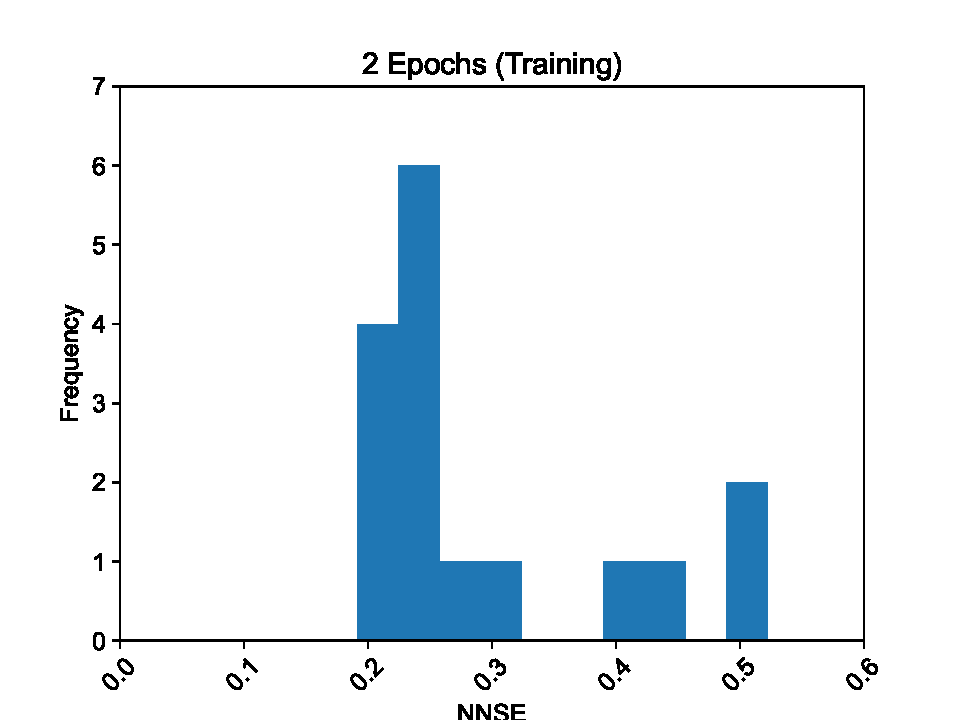
\includegraphics[width=1.0\linewidth]{images/2_training-NNSE.pdf}
        \caption{NNSE - 2 epochs}
        \label{fig:tbd1}
     \end{subfigure}
     \hfill
     \begin{subfigure}[b]{0.49\textwidth}
        \centering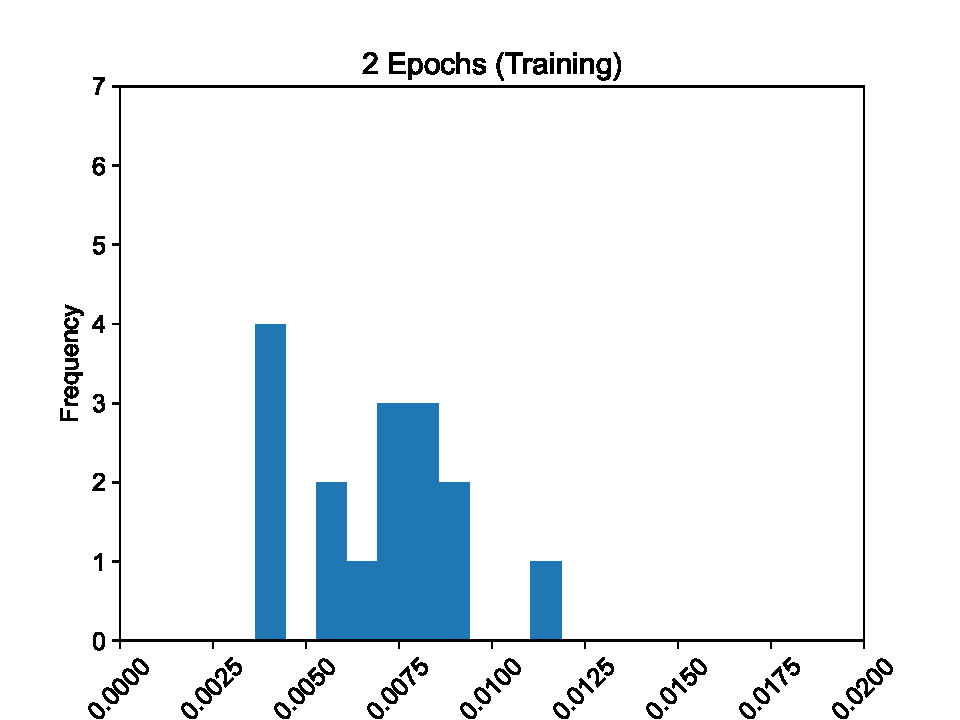
\includegraphics[width=1.0\linewidth]{images/2_training-MSE.pdf}
        \caption{MSE - 2 epochs}
        \label{fig:tbd2}
     \end{subfigure}
     \hfill
     \newline
     \begin{subfigure}[b]{0.49\textwidth}
        \centering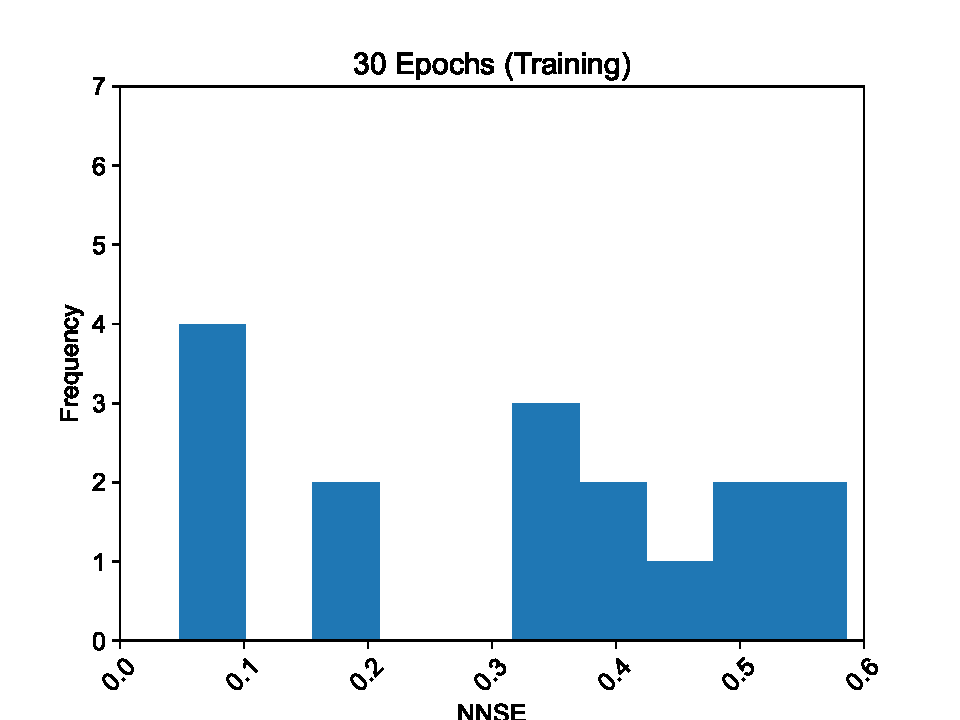
\includegraphics[width=1.0\linewidth]{images/30_training-NNSE.pdf}
        \caption{NNSE - 30 epochs}
        \label{fig:tbd3}
     \end{subfigure}
     \hfill
     \begin{subfigure}[b]{0.49\textwidth}
        \centering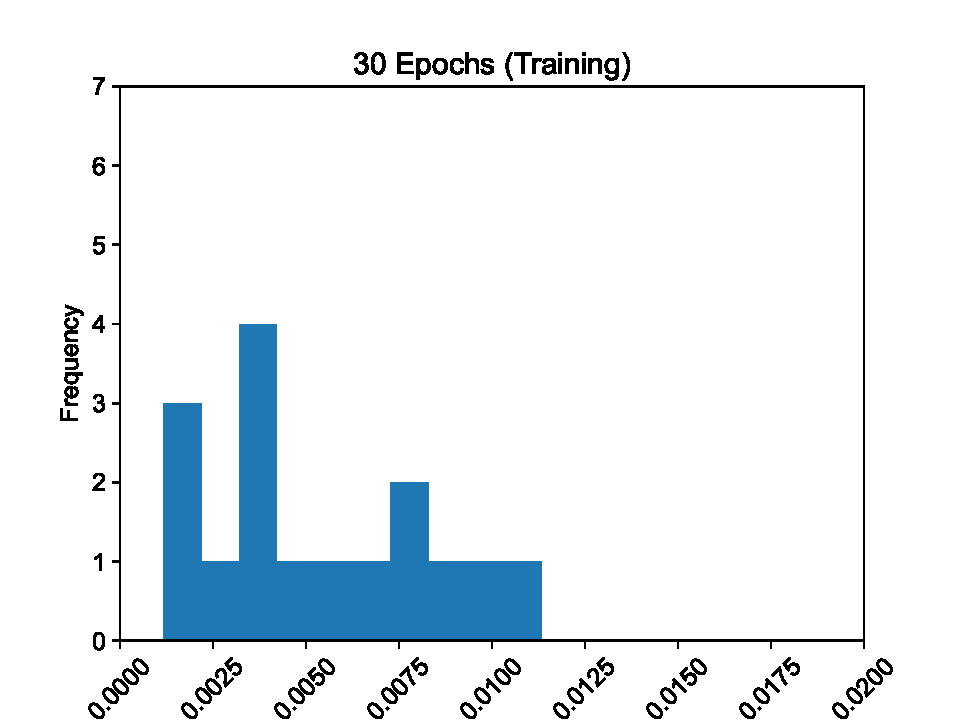
\includegraphics[width=1.0\linewidth]{images/30_training-MSE.pdf}
        \caption{MSE - 30 epochs}
        \label{fig:tbd4}
     \end{subfigure}
     \hfill
          \newline
     \hfill
     \begin{subfigure}[b]{0.49\textwidth}
        \centering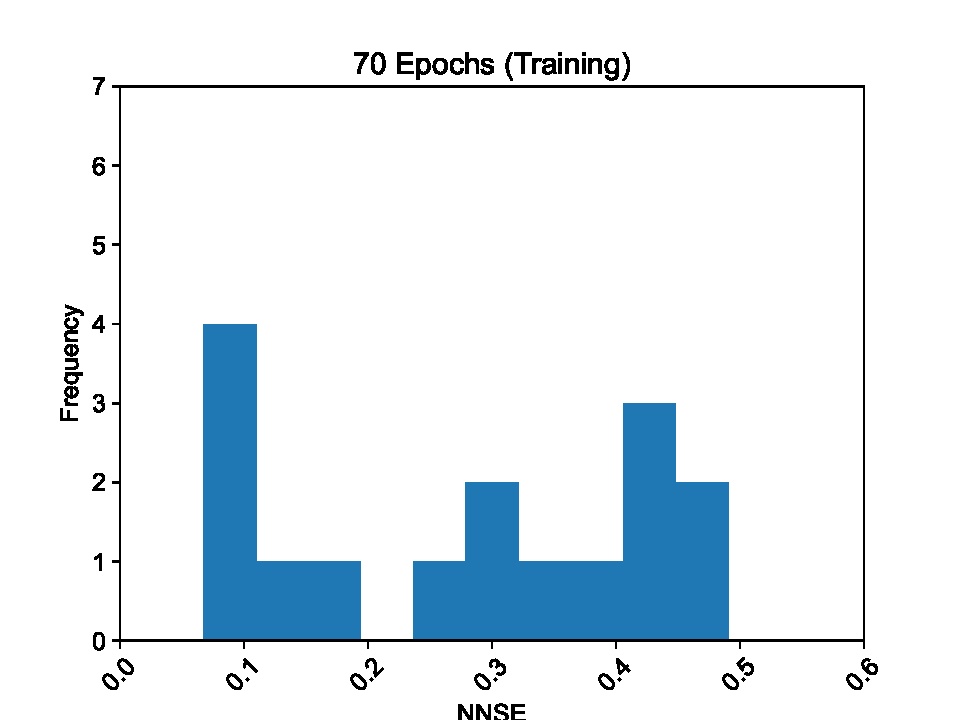
\includegraphics[width=1.0\linewidth]{images/70_training-NNSE.pdf}
        \caption{NNSE - 70 epochs}
        \label{fig:tbd3}
     \end{subfigure}
     \hfill
     \begin{subfigure}[b]{0.49\textwidth}
        \centering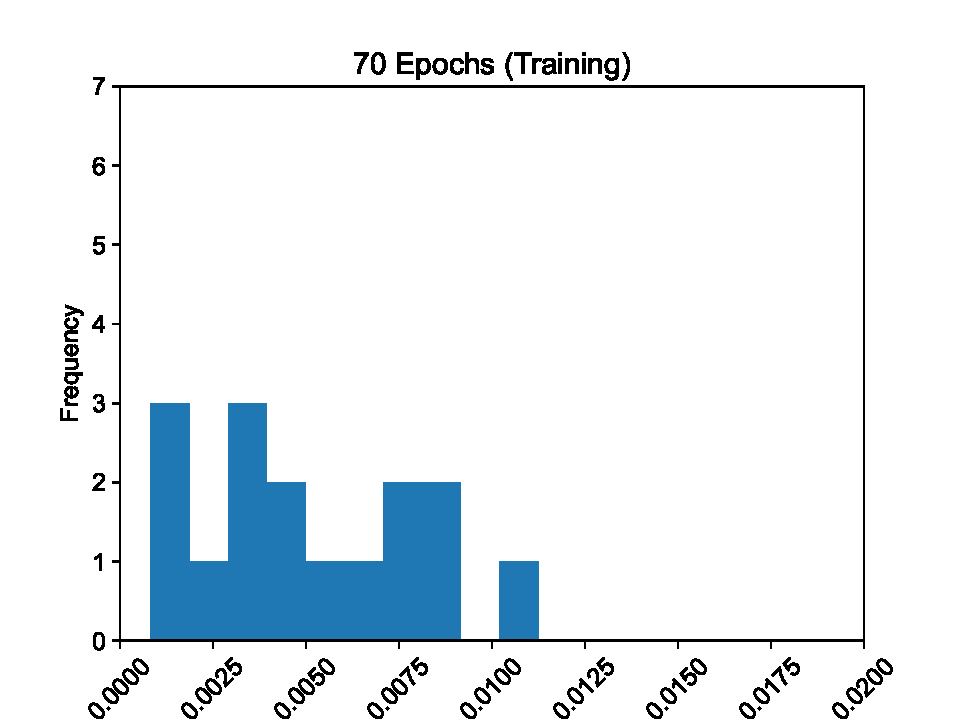
\includegraphics[width=1.0\linewidth]{images/70_training-MSE.pdf}
        \caption{MSE - 70 epochs}
        \label{fig:tbd4}
     \end{subfigure}
        \caption{NNSE and MSE values for epochs 2, 30, 70 (training).}
        \label{fig:six graphs}
\end{figure*}

\begin{figure*}[p]
     \centering
     \begin{subfigure}[b]{0.49\textwidth}
        \centering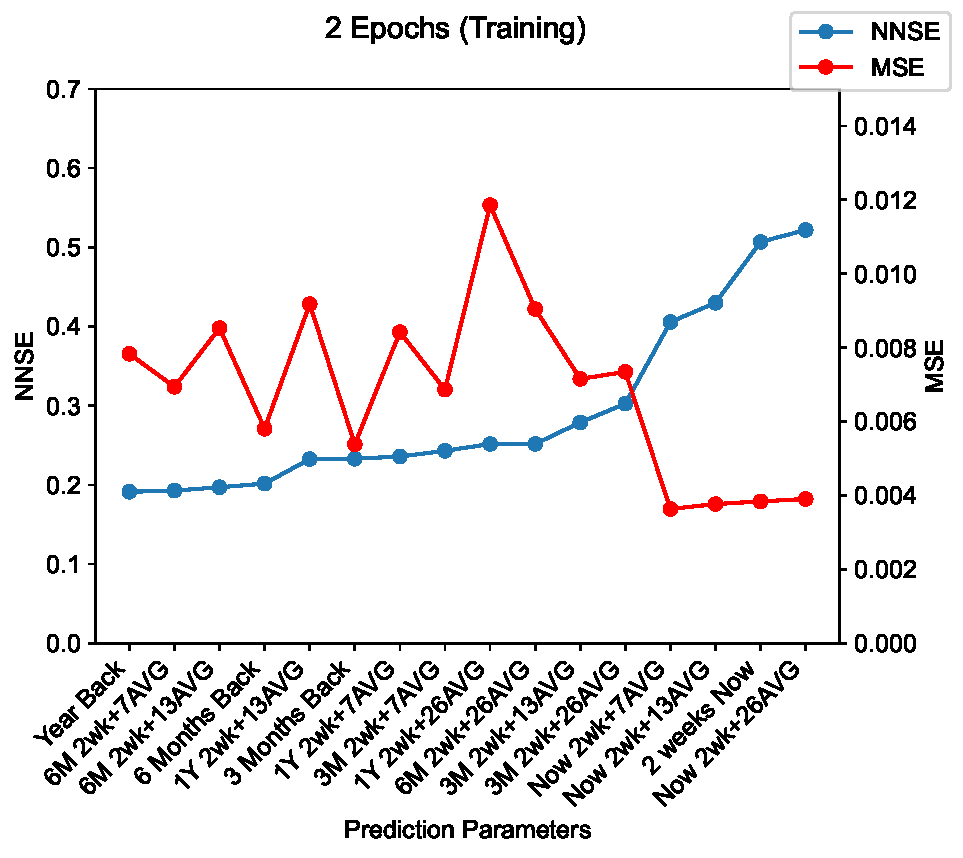
\includegraphics[width=1.0\linewidth]{images/2_training-MSE-and-NNSE.pdf}
        \caption{MSE and NNSE - 2 epochs training}
        \label{fig:tbd1}
     \end{subfigure}
     \hfill
     \begin{subfigure}[b]{0.49\textwidth}
        \centering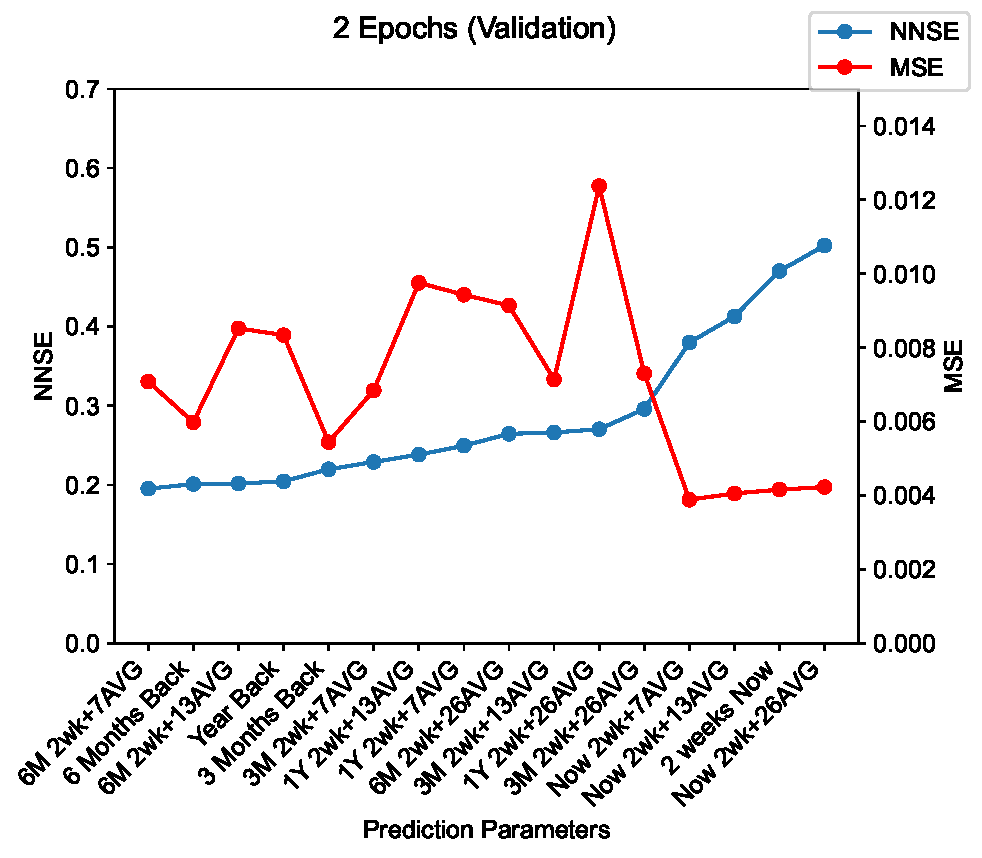
\includegraphics[width=1.0\linewidth]{images/2_validation-MSE-and-NNSE.pdf}
        \caption{MSE and NNSE - 2 epochs validation}
        \label{fig:tbd2}
     \end{subfigure}
     \hfill
     \newline
     \begin{subfigure}[b]{0.49\textwidth}
        \centering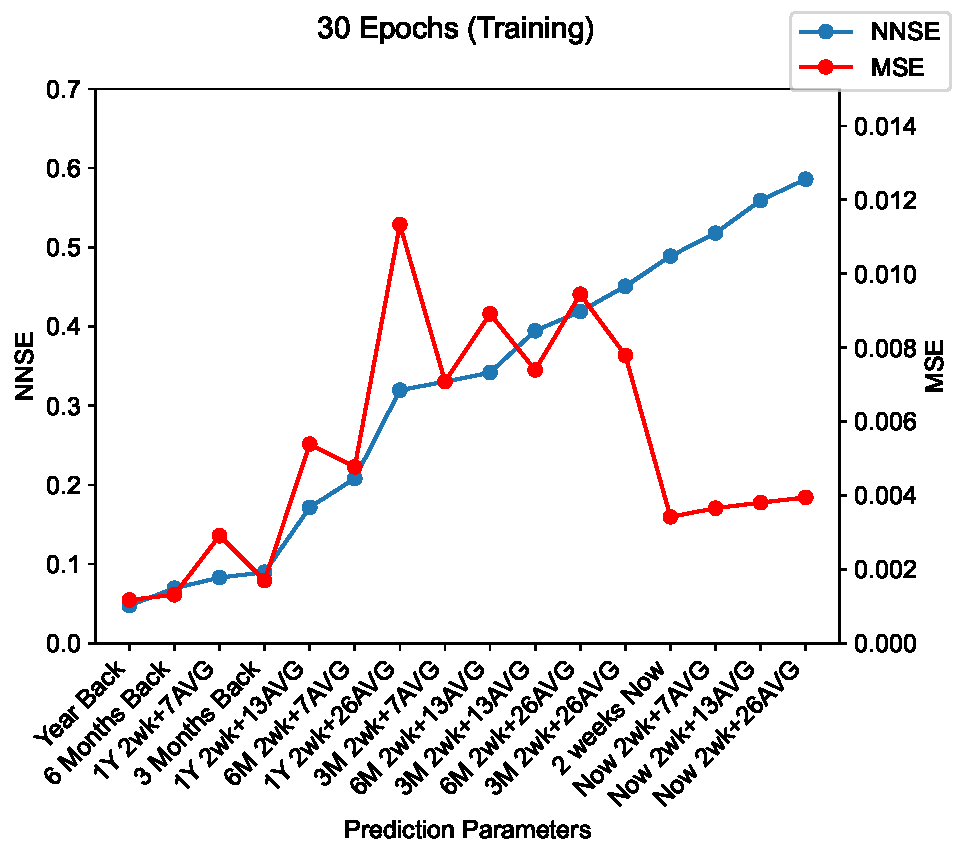
\includegraphics[width=1.0\linewidth]{images/30_training-MSE-and-NNSE.pdf}
        \caption{MSE and NNSE - 30 epochs training}
        \label{fig:tbd3}
     \end{subfigure}
     \hfill
     \begin{subfigure}[b]{0.49\textwidth}
        \centering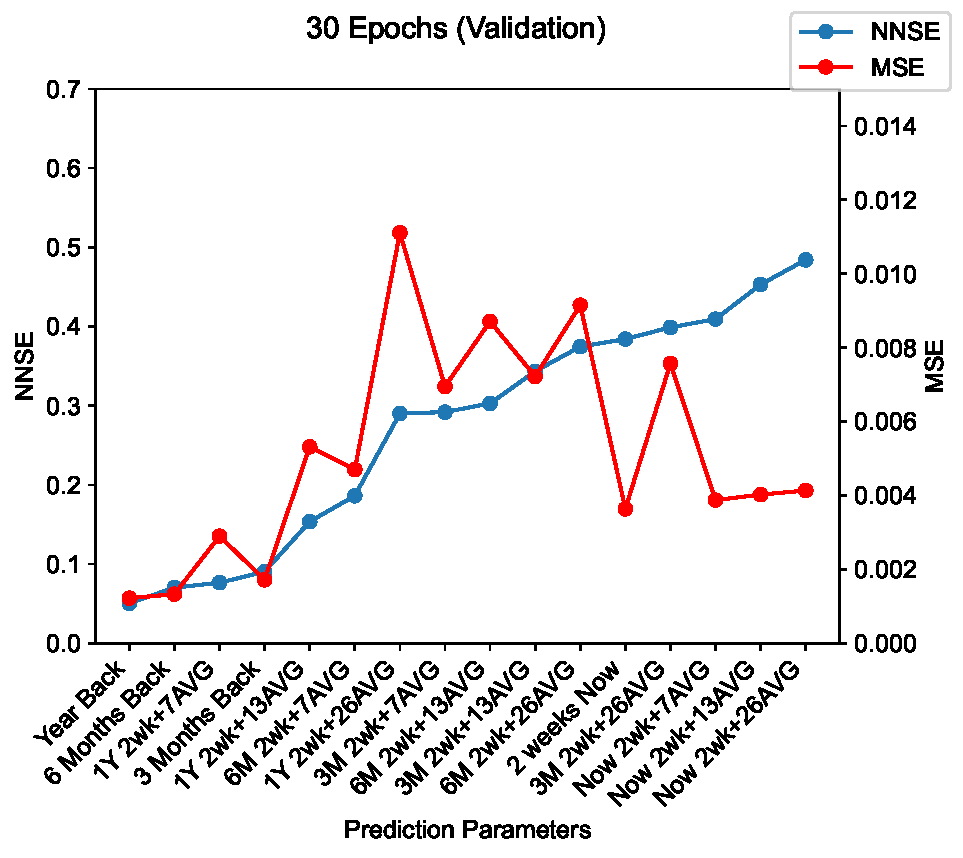
\includegraphics[width=1.0\linewidth]{images/30_validation-MSE-and-NNSE.pdf}
        \caption{MSE and NNSE - 30 epochs validation}
        \label{fig:tbd4}
     \end{subfigure}
     \hfill
          \newline
     \hfill
     \begin{subfigure}[b]{0.49\textwidth}
        \centering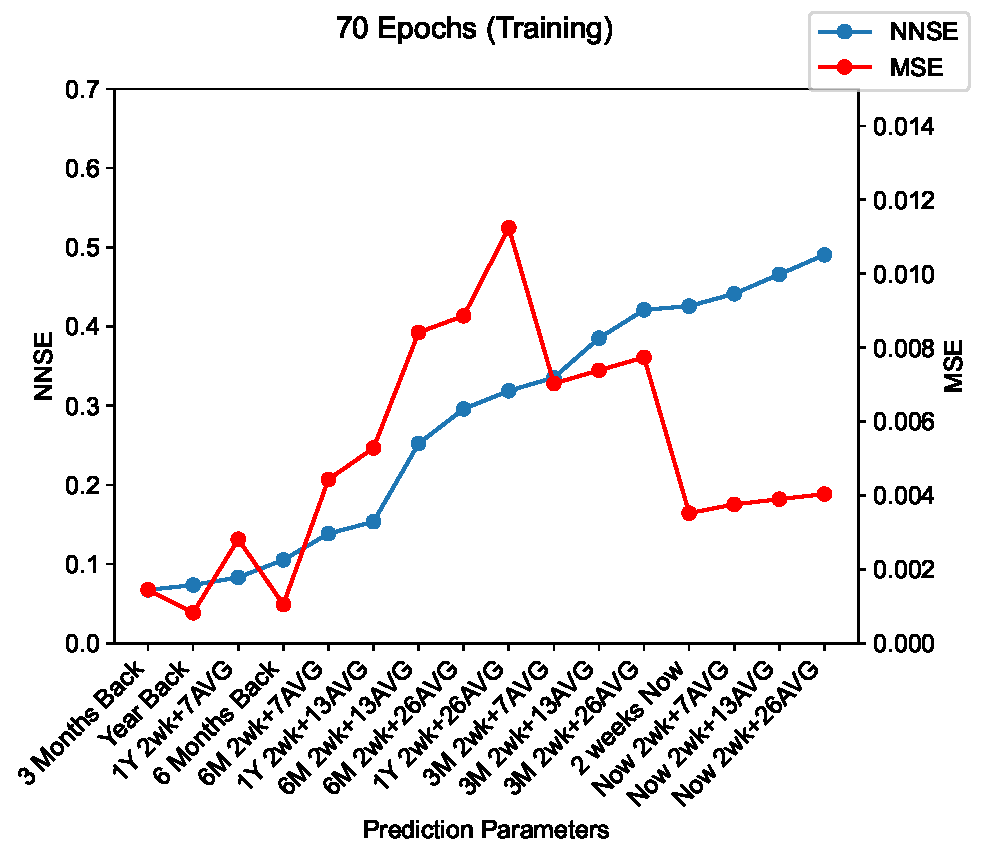
\includegraphics[width=1.0\linewidth]{images/70_training-MSE-and-NNSE.pdf}
        \caption{MSE and NNSE - 70 epochs training}
        \label{fig:tbd3}
     \end{subfigure}
     \hfill
     \begin{subfigure}[b]{0.49\textwidth}
        \centering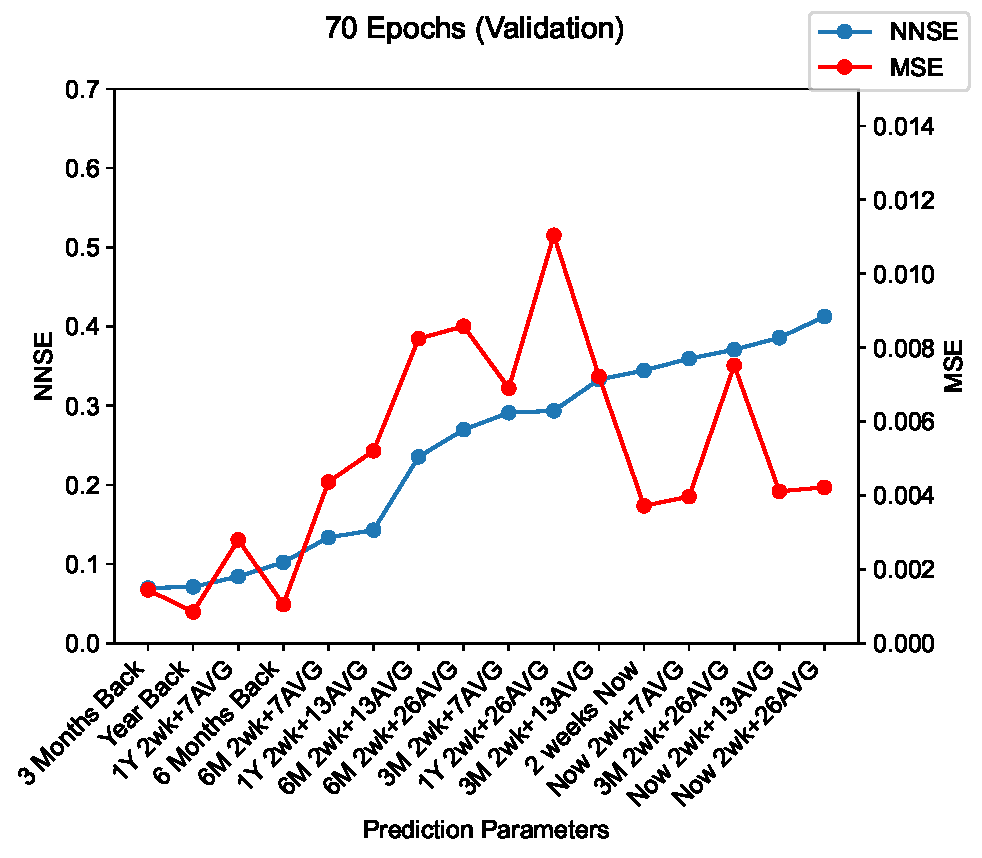
\includegraphics[width=1.0\linewidth]{images/70_validation-MSE-and-NNSE.pdf}
        \caption{MSE and NNSE - 70 epochs validation}
        \label{fig:tbd4}
     \end{subfigure}
        \caption{NNSE and MSE values for epochs 2, 30, 70 (training and validation).}
        \label{fig:six graphs}
\end{figure*}

%\begin{figure}[htb]
%%\centering\includegraphics[width=1.0\columnwidth]{usecase/images/hvac-new-arch.png}
%\centering\includegraphics[width=1.0\columnwidth]{images/2-weeks-now.pdf}
%\caption{To be determined}
%\label{fig:tbd}
%\end{figure}

\begin{table}[htb]
%\centering\includegraphics[width=1.0\columnwidth]{usecase/images/hvac-new-arch.png}

\caption{To be determined}
\label{tab:tbd}
\bigskip
%\resizebox{1.0\columnwidth}{!}{%
\centering\begin{tabular}{rl}
NNSE & name \\
\hline
0.191300 & Year Back \\
0.192700 & 6M 2wk+7AVG \\
0.197000 & 6M 2wk+13AVG \\
0.201600 & 6 Months Back \\
0.232600 & 1Y 2wk+13AVG \\
0.233000 & 3 Months Back \\
0.235800 & 1Y 2wk+7AVG \\
0.243000 & 3M 2wk+7AVG \\
0.251600 & 1Y 2wk+26AVG \\
0.251700 & 6M 2wk+26AVG \\
0.278800 & 3M 2wk+13AVG \\
0.302500 & 3M 2wk+26AVG \\
0.405600 & Now 2wk+7AVG \\
0.429900 & Now 2wk+13AVG \\
0.506800 & 2 weeks Now \\
0.521800 & Now 2wk+26AVG \\
\hline
\end{tabular}%
%}
\end{table}

\begin{table}[htb]
%\centering\includegraphics[width=1.0\columnwidth]{usecase/images/hvac-new-arch.png}

\caption{To be determined}
\label{tab:tbdetermined}
\bigskip
%\resizebox{1.0\columnwidth}{!}{%
\centering\begin{tabular}{rl}
NNSE & 2 Week Intervals \\
\hline
0.195200 & 6M 2wk+7AVG \\
0.201000 & 6 Months Back \\
0.201600 & 6M 2wk+13AVG \\
0.204500 & Year Back \\
0.219700 & 3 Months Back \\
0.228900 & 3M 2wk+7AVG \\
0.238200 & 1Y 2wk+13AVG \\
0.249500 & 1Y 2wk+7AVG \\
0.264400 & 6M 2wk+26AVG \\
0.266200 & 3M 2wk+13AVG \\
0.270300 & 1Y 2wk+26AVG \\
0.295800 & 3M 2wk+26AVG \\
0.379700 & Now 2wk+7AVG \\
0.412700 & Now 2wk+13AVG \\
0.470100 & 2 weeks Now \\
0.502300 & Now 2wk+26AVG \\
\hline
\end{tabular}%
%}
\end{table}

\section*{Acknowledgements}

Continued work was in part funded by the NSF CyberTrain-
ing: CIC: CyberTraining for Students and Technologies from
Generation Z with the award numbers 1829704 and 2200409
and NIST 60NANB21D151T.

\clearpage

\bibliographystyle{IEEEtran}
\bibliography{report}


\end{document}
